\subsection{Gestione della configurazione}
\label{subsec:gestione_della_configurazione}
Il processo di gestione della configurazione ha il compito di identificare e definire le pratiche e gli strumenti necessari per tenere traccia: delle modifiche, dello stato e dei rilasci dei componenti del sistema.

\subsubsection{Repository}
\label{subsubsec:repository}
I prodotti del progetto vengono nelle seguenti repository:
\begin{enumerate}
    \item \textbf{SorgentiDocumentazione}: \href{https://github.com/ALT-F4-eng/SorgentiDocumentazione}{https://github.com/ALT-F4-eng/SorgentiDocumentazione};
    \item \textbf{Documentazione}: \href{https://github.com/ALT-F4-eng/Documentazione}{https://github.com/ALT-F4-eng/Documentazione};
    \item \textbf{PoC}: \href{https://github.com/ALT-F4-eng/PoC}{https://github.com/ALT-F4-eng/PoC}.
\end{enumerate}
Di seguito vengono approfondito lo scopo e la struttura di tali repository.

\paragraph{SorgentiDocumentazione}
Questo \glossario{repository} contiene i sorgenti della documentazione scritti usando il linguaggio \glossario{LaTeX}.
In particolare contiene le seguenti cartelle e file:
\begin{enumerate}
    \item \textbf{Candidatura}, \textbf{RTB} e \textbf{PB}: cartelle che contengono le i documenti sorgenti definiti durante le relative fasi del progetto;
    
    \item \textbf{Workflows}: file che definiscono le automazioni associate al \glossario{repository} e vengono denominati usando la sintassi \glossario{Pascal case};
    
    \item \textbf{Immagini}: cartella che contiene il logo del gruppo;
    
    \item \textbf{Packages}: cartella che contiene la definizione del pacchetto \glossario{Latex} personalizzato utilizzato dal gruppo;
    
    \item \textbf{README.md}: file che contiene la descrizione del \glossario{repository} e del gruppo;
    
    \item \textbf{.gitignore}: file speciale che contiene una lista di file che il sistema di versionamento deve ignorare.
\end{enumerate}

\paragraph{Documentazione}
Questo \glossario{repository} contiene i file PDF prodotti dalla compilazione dei sorgenti della documentazione e i file necessari per presentarli tramite il sito web del gruppo.
Il \glossario{repository} contiene le seguenti cartelle e file:
\begin{enumerate}
    \item \textbf{Assets}: cartella che contiene tutte le immagini e le icone usate nel sito web;
    
    \item \textbf{Candidatura}, \textbf{RTB} e \textbf{PB}: cartelle che contengono i PDF dei file sorgente presenti nella relative cartelle del repository SorgentiDocumentazione;

    \item \textbf{Js}: cartella che contiene tutti i file JavaScript usati dal sito web;

    \item \textbf{Style}: cartella che contiene tutti i file CSS usati dal sito web;
    
    \item \textbf{README.md}: file che contiene la descrizione del \glossario{repository} e del gruppo;
    
    \item \textbf{index.html}: file html che corrisponde alla home page del sito web.
\end{enumerate}

\paragraph{PoC}
Questo \glossario{repository} contiene i file sorgenti del \glossario{Proof of Concept}.
Il \glossario{repository} contiene le seguenti cartelle e file:
\begin{enumerate}
    \item \textbf{back-end}: cartella che contiene tutti file sorgente che compongono la parte back-end del \glossario{PoC};
    
    \item \textbf{front-end}: cartella che contiene tutti i file sorgente che compongono la parte front-end del \glossario{PoC}.
\end{enumerate}

\subsubsection{Schema di versionamento}
Il gruppo ha deciso di utilizzare il seguente schema di versionamento per indicare le versioni dei componenti del sistema:
\begin{lstlisting}
    vX.Y
\end{lstlisting}
Dove:
\begin{enumerate}
    \item \texttt{X}: intero positivo che indica la versione major del componente.
    La versione major indica a quante volte il componente ha raggiunto uno stato ritenuto come "stabile" dal gruppo;

    \item \texttt{Y}: intero positivo che indica la versione minor del documento.
    La versione minor indica il numero di modifiche effettuate all'elemento a partire dall'ultima versione major.
\end{enumerate}

\subsubsection{Strategia di branching}
\label{subsub:branching}
Come \glossario{strategia di branching} il gruppo ha scelto l'utilizzo di \glossario{Gitflow} dato che permette di massimizzare il lavoro parallelo riducendo la complessità di risoluzione dei conflitti.
Di seguito vengono descritti i rami utilizzati da \glossario{Gitflow} e le convenzioni usate dal gruppo per la loro denominazione.
\begin{enumerate}

    \item \textbf{main}: contiene la \glossario{codeline} principale ovvero le versioni dei file che compongono l'ultima \glossario{baseline} raggiunta.
    Questo ramo è un ramo "stabile" nel senso che persiste nel \glossario{repository} lungo tutta la sua vita;

    \item \textbf{develop}: contiene la \glossario{codeline} secondaria ovvero i cambiamenti verificati che si sommeranno formando la prossima \glossario{baseline}.
    Anche questo ramo è un ramo "stabile" e viene creato a partire dal ramo main;

    \item \textbf{feature}: vengono usati dai membri del gruppo per implementare le modifiche.
    Sono dei rami "provvisori" nel senso che esistono finché il loro contenuto non viene verificato.
    I rami feature vengono creati a partire dal ramo develop e confluiscono in esso quando il loro contenuto passa con successo la verifica.
    Il gruppo ha deciso di utilizzare la seguente convenzione per la denominazione di questi rami:
    \begin{lstlisting}
        feature/#<id issue>
    \end{lstlisting}
    Così facendo si ottiene un collegamento immediato tra ramo di feature e richiesta di modifica;

    \item \textbf{hotfix}: usati per eseguire modifiche rapide e di dimensioni ridotte.
    Queste modifiche non influenzano quindi le versioni dei componenti del sistema.
    Questi rami sono "provvisori" nel senso che vengono eliminati dopo che le loro modifiche sono state allineate ai rami main e develop;


    \item \textbf{release}: usati dal Responsabile del gruppo per approvare il contenuto del ramo develop consolidandolo in una \glossario{baseline} nella \glossario{codeline} principale.
    Sono dei rami "provvisori" nel senso che esistono finché il loro contenuto non viene approvato.
    I rami release vengono creati a partire dal ramo develop e confluiscono nei rami main e develop.
    Il gruppo ha deciso di utilizzare la seguente convenzione per la denominazione di questi rami:
    \begin{lstlisting}
        release/<nome milestone>
    \end{lstlisting}
    Così facendo si ottiene un collegamento immediato tra ramo di release e la \glossario{milestone} che raggiunge.
\end{enumerate}
I comandi base necessari per applicare questa strategia di branching sono:
\begin{lstlisting}    
    // eseguire commit con messaggio
    git commit -m "<messaggio>" 

    // fusione ramo corrente con ramo indicato
    git merge <ramo>

    // gestione staging area
    git add <lista file>
    git rm <lista file>

    // importa modifiche da repository remoto
    git push origin <ramo>

    // pubblica modifiche sul repository remoto
    git pull origin <ramo>
\end{lstlisting}

\subsubsection{Gestione delle richieste di modifica}
Il gruppo per gestire le richieste di modifica ha deciso di utilizzare le funzionalità offerte da \glossario{GitHub}.

\paragraph{Issue}
\glossario{GitHub} fornisce un \glossario{ITS} ovvero un sistema che permette di registrare e gestire le richieste di modifica.
Le richieste di modifica sono rappresentate tramite il concetto di issue.
Un \glossario{issue} è composta dai seguenti elementi:
\begin{enumerate}
    \item \textbf{Titolo}: nome della richiesta di modifica;
   
    \item \textbf{Id}: identifica univocamente la richiesta di modifica;
   
    \item \textbf{Stato}: stato attuale della richiesta di modifica tra gli stati che essa può attraversare durante il suo \glossario{ciclo di vita};
   
    \item \textbf{Etichetta}: tipologia di richiesta di modifica;
   
    \item \textbf{Assegnatario}: membro del gruppo di lavoro che ha la responsabilità di implementare la richiesta di modifica;
    
    \item \textbf{Verificatore}: membro del gruppo di lavoro responsabile per la verifica dell'implementazione della richiesta di modifica;
   
    \item \textbf{Milestone}: \glossario{milestone} a cui la richiesta di modifica appartiene;
   
    \item \textbf{Descrizione}: specifica con più precisione la richiesta di modifica.
\end{enumerate}

\subparagraph{Etichette}
Di seguito viene fornita una lista delle etichette utilizzate dal gruppo:
\begin{enumerate}
    \item \textbf{bug}: riguarda la correzione di un documento o di un errore presente nel codice;
    
    \item \textbf{enhancement}: riguarda l'implementazione di automazioni della gestione e organizzazione di progetto o il miglioramento del codice;
    
    \item \textbf{requirement}: riguardano il documento di analisi dei requisiti;
    
    \item \textbf{feature}: riguarda l'implementazione di una nuova funzionalità;

    \item \textbf{documentation}: riguardano lo sviluppo di altri documenti.
\end{enumerate}

\subparagraph{Stato}
Lo stato di una \glossario{issue} è una proprietà personalizzata che corrisponde allo stato della richiesta di modifica che la \glossario{issue} rappresenta.
I valori che questa proprietà può assumere sono:
\begin{enumerate}
    \item \textbf{To do}: il membro del team che ha la responsabilità di implementare la richiesta di modifica deve ancora iniziare a lavorarci;
    
    \item \textbf{In progress}: il membro del team che ha la responsabilità di implementare la richiesta di modifica ci sta lavorando;
    
    \item \textbf{To review}: il verificatore designato deve ancora iniziare la verifica dell'implementazione;
    
    \item \textbf{In review}: il verificatore designato sta verificando l'implementazione;
    
    \item \textbf{Re open}: il verificatore designato ha ritenuto l'implementazione non all'altezza delle aspettative.
    L'implementazione deve quindi essere migliorata dal membro del team responsabile;
    
    \item \textbf{Done}: il verificatore ha accettato l'implementazione.
\end{enumerate}


\paragraph{Ciclo di vita delle issue}
Gli stati che una issue attraversa durante il suo \glossario{ciclo di vita} sono riassunti nel diagramma in \hyperref[fig:ciclo_di_vita]{Figura \ref{fig:ciclo_di_vita}}.
\begin{figure}[H]
    \center
    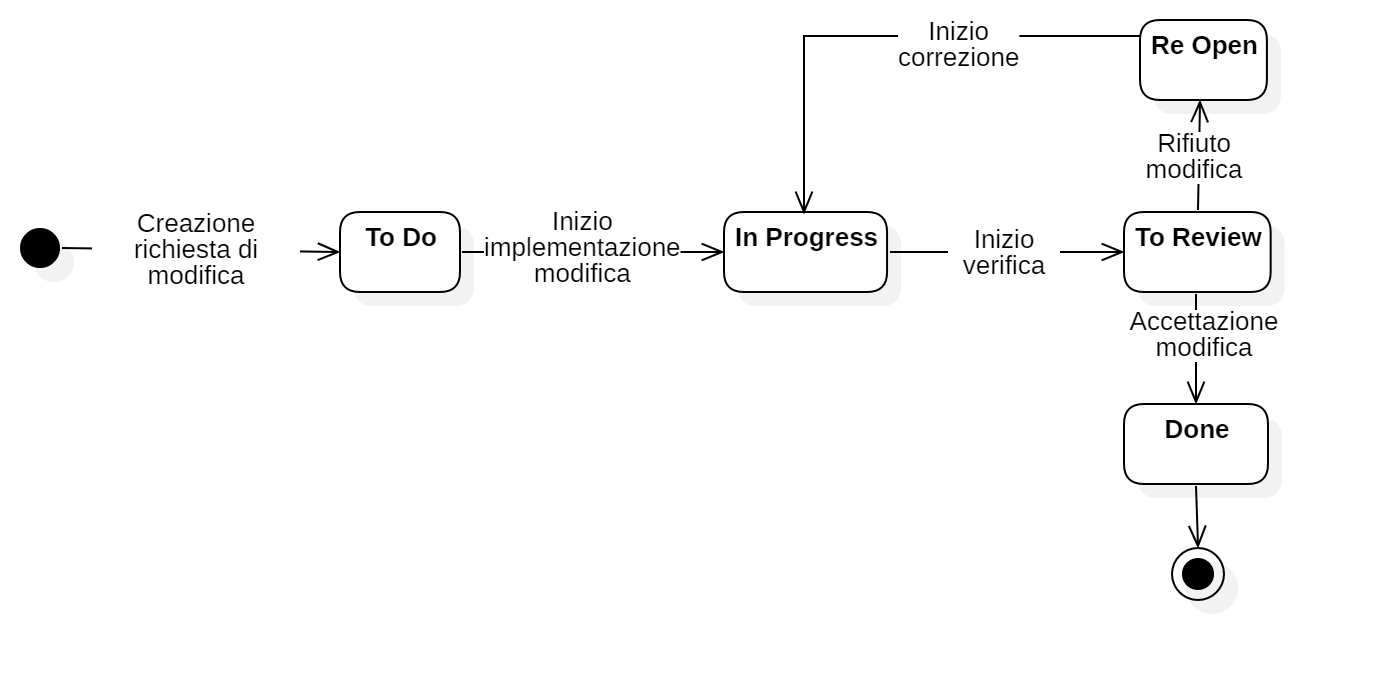
\includegraphics[scale=0.25]{Sezioni/ProcessiDiSupporto/Immagini/cicloDiVita.png}
    \caption{Ciclo di vita di una issue}
    \label{fig:ciclo_di_vita}
\end{figure}
Per visualizzare l'andamento delle issue definite il gruppo ha deciso di utilizzare una board di progetto che organizza le issue definite in colonne basandosi sul loro stato.
Un membro che ha svolto un compito che fa "avanzare" una issue nel suo ciclo di vita deve quindi interagire con la board.
Alcune di queste interazioni sono state automatizzate.
Di seguito vengono elenecate le azioni che permettono la modifica dello stato di una issue. 

\subparagraph{Richiesta di verifica}
Per richiedere la verifica di una modifica è necessario aprire una \glossario{pull request} dove:
\begin{itemize}
    \item \textbf{Ramo sorgente}: contiene la modifica da verificare.
    \item \textbf{Ramo destinazione}: il ramo develop.
\end{itemize}

\subparagraph{Presa in carico di una verifica}
Per poter prendere in carico una verifica essa deve essere nello stato To Review e quindi risiedere nella relativa colonna della board.
Per prendere in carico una verifica il Verificatore deve trascinare la issue dalla colonna To Review alla colonna In Review.


\subparagraph{Accettazione modifiche}
Per accettare le modifiche di cui è stata richiesta la verifica il Verificatore deve accettare la \glossario{pull request} e integrare le modifiche nel ramo delevop.
Dopo aver accettato le modifiche il Verificatore deve eliminare il ramo che le conteneva.

\subparagraph{Rifiuto modifiche}
Per rifiutare le modifiche di cui è stata richiesta la verifica il Verificatore deve chiudere la relativa \glossario{pull request}.
Il verificatore in questo caso ha l'onere di indicare in un commento della \glossario{issue} i miglioramenti da apportare alla modifica affinchè venga accettata nella verifica successiva.


\paragraph{Registro delle modifiche}
Il gruppo ha deciso di dotare alcuni documenti di una tabella chiamata registro delle modifiche.
Questo permette di avere una storia delle versioni coerente anche nel caso in cui avvengano errori nella gestione del repository.
Di seguito viene indicata la struttura del registro delle modifiche:
\begin{enumerate}
    \item \textbf{Versione}: versione del documento dopo la verifica della modifica;
    \item \textbf{Data}: data in cui è avvenuta la modifica;
    \item \textbf{Autore/i}: nome e cognome dei componenti del gruppo che hanno eseguito le modifiche;
    \item \textbf{Verificatore/i}: nome e cognome dei verificatori (aggiornato solo dopo seguito l'accettazione della modifica);
    \item \textbf{Descrizione}: lista di link alle sezioni modificate.
    La descrizione permette ai membri del team di capire velocemente la necessità di allinearsi a nuove informazioni. 
\end{enumerate} 
\textbf{Nota bene}: Le righe del registro delle modifiche sono ordinate per versione decrescente.

\subsubsection{Rilascio}
Di seguito viene documentata l'attività di rilascio dei file che devono essere consolidati in una \glossario{baseline}.
Il rilascio deve essere eseguito dal Responsabile del team e prevede le seguenti operazioni:
\begin{enumerate}

    \item Creazione ramo release seguendo le regole indicate nella sezione \hyperref[subsub:branching]{Strategia di branching};
    
    \item Eseguire eventuali modifiche correttive minori che non riguardano il contenuto;

    \item Registrare le modifiche nel repository locale seguendo le regole indicate nella sezione  \hyperref[subsub:branching]{Strategia di branching};
    
    \item Associare un tag che identifica la baseline raggiunta;
    
    \item Registrare le modifiche nel repository remoto.
\end{enumerate}

\paragraph{Compilazione dei documenti sorgente}
La compilazione dei documenti avviene in modo automatico a ogni rilascio eseguito nella repository SorgentiDocumentazione.
Il meccanismo usato per automatizzare la compilazione è quello delle \glossario{GitHub action}.


\paragraph{Distribuzione dei documenti}
La distribuzione dei documenti avviene mediante l'utilizzo di un sito web vetrina disponibile al link \href{https://alt-f4-eng.github.io/Documentazione/}{https://alt-f4-eng.github.io/Documentazione/}.
Il contenuto del sito viene aggiornato in automatico e quindi rispecchia l'ultima compilazione automatica eseguita. 

\subsubsection{Strumenti}
Qui vengono elencati gli strumenti usati, che vengono poi approfonditi nella sezione \hyperref[sec:strumenti]{Strumenti}.
\begin{itemize}
    \item GitHub;
    \item Git.
\end{itemize}

